\documentclass[10pt]{article}

\usepackage{hyperref} 
\usepackage{graphicx} 
\usepackage{fancybox} 
\usepackage{rotating} 
\usepackage{color}  
\usepackage{here}

\ifx\MARaBOU\undefined
\def\MARaBOU{MAR\lower.5ex\hbox{a}BO\kern-.5em\lower.5ex\hbox{O}\kern-.1em U}%
\fi

\newcommand{\samefootnote}{$^\alph{footnote}$}
\newcommand{\samempfootnote}{$^\alph{mpfootnote}$}

\definecolor{lightblue}{rgb}{.68,.88,.90}

\newcommand{\blue}[1]{\colorbox{lightblue}{\texttt{#1}}}
\newcommand{\yellow}[1]{\colorbox{yellow}{\texttt{#1}}}
\newcommand{\redt}[1]{\textcolor{red}{\texttt{#1}}}
\newcommand{\greent}[1]{\textcolor{green}{\texttt{#1}}}
\newcommand{\bluet}[1]{\textcolor{blue}{\texttt{#1}}}
\newcommand{\boldt}[1]{\textbf{\texttt{#1}}}

\newenvironment{boxed}
	{\begin{Sbox}\begin{minipage}[t]}
	{\end{minipage}\end{Sbox}\fbox{\TheSbox}}
	
\newenvironment{yellowboxed}
	{\begin{Sbox}\begin{minipage}[t]}
	{\end{minipage}\end{Sbox}\colorbox{yellow}{\TheSbox}}
	
\newenvironment{blueboxed}
	{\begin{Sbox}\begin{minipage}[t]}
	{\end{minipage}\end{Sbox}\colorbox{lightblue}{\TheSbox}}
	

\setlength{\parindent}{0pt}

\begin{document}
\begin{titlepage}
\title{Instructions how to use the DAQ in a MINIBALL experiment}
\author{R. Lutter}
\maketitle
\vfill
\begin{abstract}
\setlength{\parindent}{0pt}
\begin{center}
This document describes how to use the \MARaBOU{} data acquisition system\\
in a \mbox{MINIBALL} experiment.
\end{center}
\end{abstract}
\vfill
\end{titlepage}
\newpage
\tableofcontents
\newpage
\section{Getting started}\label{GettingStarted}
\subsection{Login to the DAQ computer}\vspace{3mm}

To login into the DAQ computer do:\vspace{4mm}\\
At CERN:
\centerline{\yellow{ssh miniball@pcepuis20.cern.ch}}
or at Cologne:
\centerline{\yellow{ssh miniball@minidaq.ikp.uni-koeln.de}}\\

Make sure that your working directory is the one prepared for the current experiment.\\
A \yellow{pwd} command should give something like \texttt{/d1/miniball/<my\_working\_directory>}:\\
\hspace*{.2\linewidth}\yellow{/d1/miniball/cern-040719} for example\\

Use \yellow{cd /d1/miniball/<my\_working\_directory>} in case you are in the wrong place.\\
\bluet{To start a new session in a new working directory refer to \ref{CreateNewDir} }.\\

From now on it is assumed that you are logged into the DAQ computer. 

\subsection{How to set up and control a list-mode run}\label{SetupListmodeRun}\vspace{3mm}

To learn how to generate your code and to compile analysis and readout parts, respectively, see \ref{GenerateAndCompileCode}.\\

To start the control GUI type:\\

\hspace*{.2\linewidth}\yellow{C\_analyze}\\

Once the GUI has popped up (fig. \ref{CanalyzeGUI}) you should check if all settings are as expected:\\
\begin{center}
\begin{itemize}
\setlength{\rightmargin}{1em}%
\setlength{\leftmargin}{2em}%
\setlength{\itemsep}{0pt}%
\setlength{\parskip}{1mm}%
\setlength{\partopsep}{0pt}%
\setlength{\parsep}{0pt}%
\setlength{\topsep}{0pt}%
\item	Set \blue{RUN} number appropriate. It will be incremented after each run.
\item	Choose \blue{TcpIp} to connect to the PowerPC and the \texttt{VME} crate.
\item	Choose \texttt{ppc-0} from the \blue{Master} list.\\
	This will set the \blue{Readout} processor to \texttt{ppc-0} automatically.
\item	Set \blue{Directory} to \texttt{<my\_working\_directory>/ppc}
\item	The name of the \texttt{ROOT} file to store histograms should be \texttt{histsRUN.root},\\
	\texttt{RUN} will on start be substituted by the current run number.
\item	Set \blue{Mapped name} to \texttt{none}
\item	Enable or disable raw data output. The name of the output file should be \texttt{runRUN.med},\\
	extension \texttt{.med} is mandatory to produce med formatted data.
\end{itemize}
\end{center}

If you made some changes to these settings you should save them pressing (fig. \ref{CanalyzeSaveSetup})\\

\hspace*{.2\linewidth}\blue{Save Setup}$\rightarrow$\blue{Save current settings}\\

Now press\\

\hspace*{.2\linewidth}\blue{Clear MBS}\\

This should stop all pending \texttt{MBS} processes and put \texttt{MBS} into an idle state.
You should end up with the message\\
\hspace*{.2\linewidth}\greent{c\_ana: Ok, all \texttt{MBS} processes disappeared}\\

In case of problems you have to reset \texttt{MBS} manually (see \ref{ResetMBSManually}).
\newpage
\begin{figure}[H]
\centerline{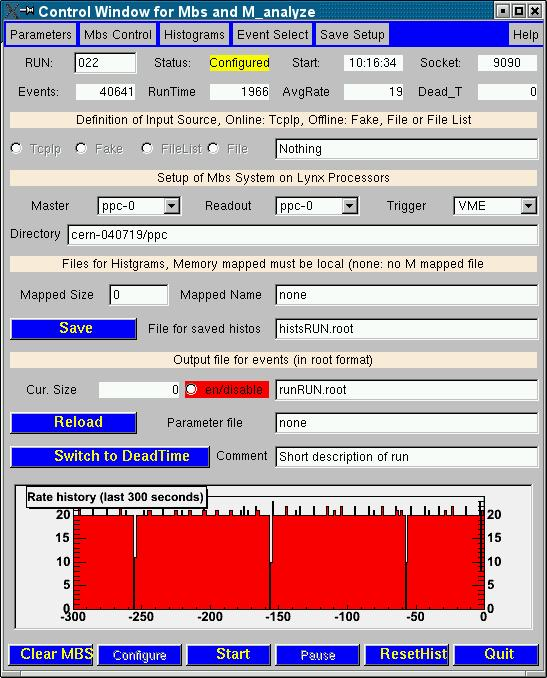
\includegraphics[width=.9\linewidth]{C_analyzeGUI}}
\caption{\texttt{C\_analyze} - GUI to control a list-mode run}
\label{CanalyzeGUI}
\end{figure}
\begin{figure}[H]
\centerline{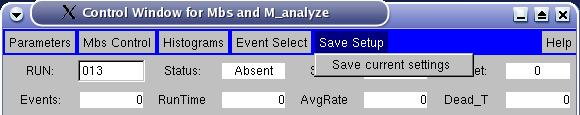
\includegraphics[width=\linewidth]{C_analyzeSaveSetup}}
\caption{\texttt{C\_analyze}: how to save setup}
\label{CanalyzeSaveSetup}
\end{figure}
\newpage
To configure \texttt{MBS} for your experiment press\\

\hspace*{.2\linewidth}\blue{Configure}\\

After having selected wether a file should be written or not press\\

\hspace*{.2\linewidth}\blue{Start}\\

To stop the run press\\

\hspace*{.2\linewidth}\blue{Stop}\\

This will close the list-mode data file and write all histograms to a \texttt{ROOT} file.

\subsection{How to run in AutoFile mode}\vspace{3mm}

As file sizes are restricted to \texttt{2\,GB} one has to keep files at sizes below this limit.\\
You may activate the \texttt{AutoFile} mode to split the raw data stream into several files in a production run.
Choose from the menu bar (fig. \ref{CanalyzeSetFileSize}) \\

\hspace*{.2\linewidth}\blue{Parameters}$\rightarrow$\blue{Maximum output file size}\\

insert the value you want in MB, then activate\\

\hspace*{.2\linewidth}\blue{Parameters}$\rightarrow$\blue{Enable automatic restart after max file size}\\

This will cause \texttt{C\_analyze} to stop the run as soon as the given file size is reached and to
continue with the next run (run number will be increased).\\
As the size check is done every second you should set the maximum file size a true bit below
the limit of \texttt{2\,GB} (let's say to \texttt{1800}) to give \texttt{C\_analyze} a chance to
stop before the limit is reached. Otherwise the resulting file may be truncated.\\

To leave \texttt{AutoFile} mode simply press \blue{Stop}.

\begin{figure}[H]
\centerline{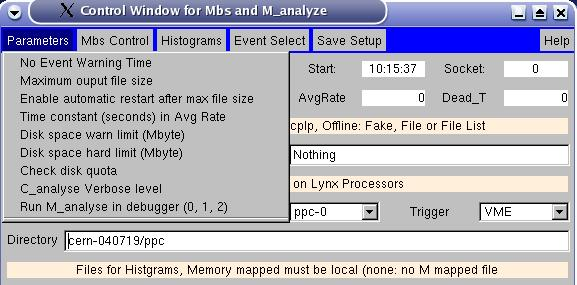
\includegraphics[width=\linewidth]{C_analyzeSetFileSize}}
\caption{\texttt{C\_analyze}: how to set autoFile mode}
\label{CanalyzeSetFileSize}
\end{figure}
\newpage
\subsection{Display of scaler data}\label{ScalerData}\vspace{3mm}

To display contents of the \texttt{VME} scalers as well as the internal dgf scalers\\
open two separate \texttt{xterm} windows. Then type\\

\hspace*{.2\linewidth}\yellow{scaler.sh} (\textbf{without} preceeding "./"!)\\

to display the \texttt{VME} scalers, and\\

\hspace*{.2\linewidth}\yellow{dgfscaler.sh} (\textbf{without} preceeding "./"!)\\

to display dgf scalers, respectively.\\
Scaler data on the screen will be updated every second.

\begin{center}
\begin{minipage}[t]{.6\linewidth}
\begin{figure}[H]
\centerline{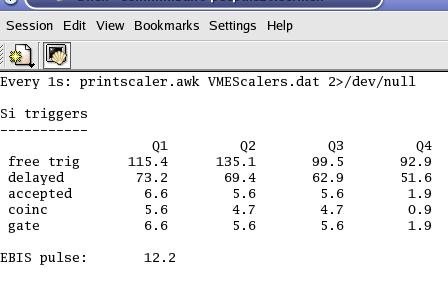
\includegraphics[width=\linewidth]{ScalerPanel.jpg}}
\caption{\texttt{Display of scaler data}}
\label{ScalerPanel}
\end{figure}
\end{minipage}
\end{center}
\begin{center}
\begin{minipage}[t]{.8\linewidth}
\begin{figure}[H]
\centerline{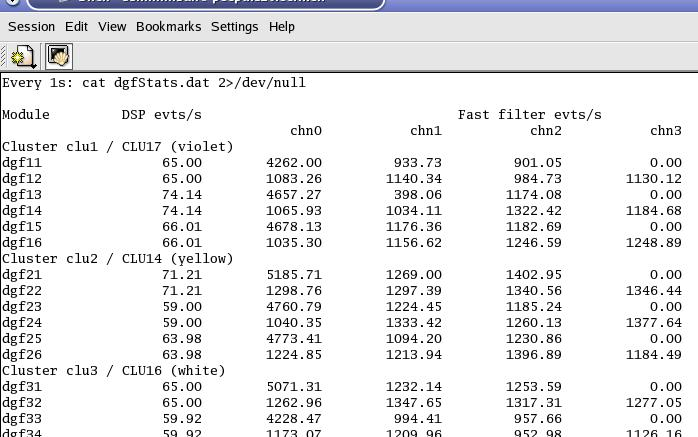
\includegraphics[width=\linewidth]{DgfScalerPanel.jpg}}
\caption{\texttt{Display of internal dgf scalers}}
\label{DgfScalerPanel}
\end{figure}
\end{minipage}
\end{center}

\subsection{PPAC beam monitor}\label{PPAC}\vspace{3mm}

To show the PPAC profile simply type\\

\hspace*{.2\linewidth}\yellow{ppac.C}\\

This will display PPAC currents for X and Y strips, respectively, with a repetition rate of 1 per second.

\begin{center}
\begin{figure}[H]
\centerline{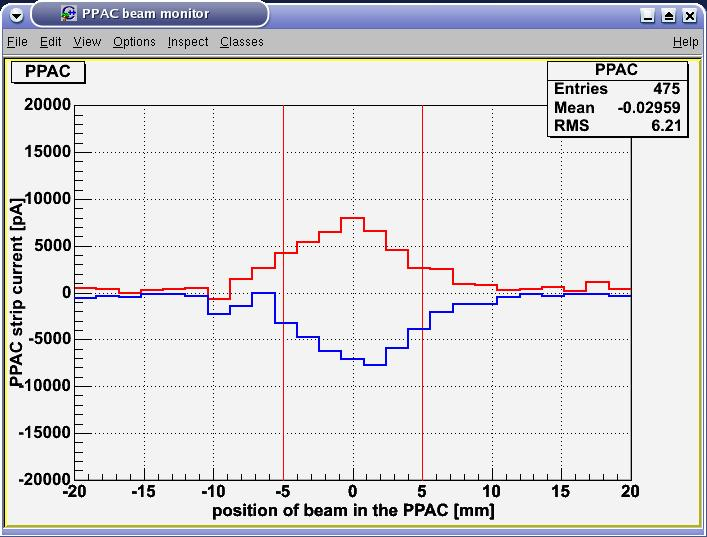
\includegraphics[width=\linewidth]{PpacBeamMonitor}}
\caption{\texttt{PPAC beam monitor}}
\label{PpacBeamMonitor}
\end{figure}
\end{center}
\newpage
\subsection{Beam rate monitor}\label{RateMon}\vspace{3mm}

To start the rate monitor type\\

\hspace*{.2\linewidth}\yellow{rateMon.C}\\

It displays counting rates for DGF cores as well as the beam dump detector.
An alarm may be triggered if the rate goes below a given threshold.\\

Counting rates are taken from a file produced by function \yellow{TUsrEvtReadout::PeakCheck()} in the online daq process
(see code in file \texttt{udef/BuildEvent.cxx}). It integrates data in two windows given by definitions in \yellow{.rootrc}:

\begin{center}
\begin{blueboxed}{.75\linewidth}
\verb+	TMrbAnalyze.PeakCheck.eMin: 276+\\
\verb+	TMrbAnalyze.PeakCheck.eMax: 282+\\
\verb+	TMrbAnalyze.PeakCheck.ratioFact: 1+\\
\verb+	TMrbAnalyze.PeakCheck.eMin2: 639+\\
\verb+	TMrbAnalyze.PeakCheck.eMax2: 632+\\
\verb+	TMrbAnalyze.PeakCheck.ratioFact2: 1+
\end{blueboxed}
\end{center}

Therefore one has to set these values properly before starting the daq process.\\

\yellow{rateMon.C} provides the following commands:
\begin{center}
\begin{tabular}{llll}
\multicolumn{4}{l}{\blue{start(range, avgShort, avgLong [, withBeamDump])}}\\
	&	\multicolumn{3}{l}{start rate display for DGF cores (and beam dump detector)}\\
	&	\boldt{range}	&	history/histogram range (s)\\
	&	\boldt{avgShort}	&	average time (s) - short term\\
	&	\boldt{avgLong}	&	average time (s) - long term\\
	&	\boldt{withBeamDump}	&	show beam dump rates if \texttt{kTRUE}\\
\blue{stop()}	&	\multicolumn{3}{l}{stop display}\\
\blue{cont()}	&	\multicolumn{3}{l}{continue display}\\
\multicolumn{4}{l}{\blue{startwd(thresh, avgTime)}}\\
	&	\multicolumn{3}{l}{start watchdog to trigger alarm if beam below threshold}\\
	&	\boldt{thresh}	&	trigger threshold for "beam low" alarm\\
	&	\boldt{avgTime}	&	average time (s)\\
\blue{stopwd()}	&	\multicolumn{3}{l}{stop watchdog}\\
\blue{bye()}	&	\multicolumn{3}{l}{exit program}\\
\end{tabular}
\end{center}

Any of these commands may be given after the ROOT prompt manually. To start automatically with predefined settings you may
create a startup file named \yellow{.rateMon.rc} in your working directory:\\

\begin{center}
\begin{blueboxed}{.75\linewidth}
\verb+	{+\\
\verb+         start(100, 17, 84, kFALSE);+\\
\verb+         startwd(1000, 19);+\\
\verb+	}+
\end{blueboxed}
\end{center}

(Keep in mind: ROOT commands have to be enclosed in curly braces \verb+{+\dots\verb+}+!)\\

In this example \yellow{rateMon.C} will automatically start the rate display:
\begin{itemize}
\setlength{\rightmargin}{1em}%
\setlength{\leftmargin}{2em}%
\setlength{\itemsep}{0pt}%
\setlength{\parskip}{1mm}%
\setlength{\partopsep}{0pt}%
\setlength{\parsep}{0pt}%
\setlength{\topsep}{0pt}%
	\item[-]	history range is \texttt{100}
	\item[-]	averaging will be done over \texttt{17} and \texttt{84} seconds, respectively
	\item[-]	as there is no beam dump detector in the experimental setup only core rates will be displayed
	\item[-]	if core rates go below a threshold of \texttt{1000} averaged over \texttt{19} seconds an alarm will be issued
\end{itemize}
\newpage
\subsection{Laser on/off monitor}\vspace{3mm}

To show the laser on/off scaler data type\\

\hspace*{.2\linewidth}\yellow{laser.C}\\

This will give you a plot of the laser data over the last 20 minutes with a binning of 4 seconds.

\begin{center}
\begin{figure}[H]
\centerline{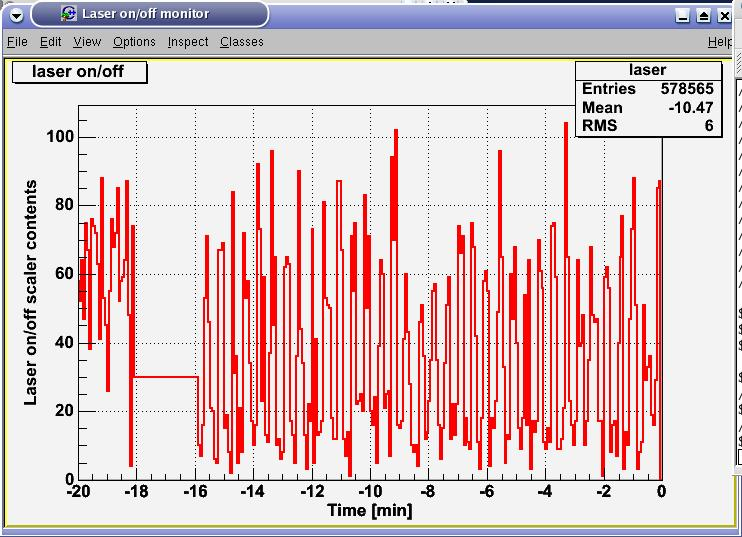
\includegraphics[width=\linewidth]{LaserMonitor}}
\caption{\texttt{Laser on/off monitor}}
\label{LaserMonitor}
\end{figure}
\end{center}
\newpage
\subsection{Display of histograms}\vspace{3mm}

To look at spectra you have to start the Histogram Presenter:\\

\hspace*{.2\linewidth}\yellow{HistPresent}\\

To connect to a running \texttt{C\_analyze} click on \blue{Hists from M\_analyze}.\\

\hspace*{.2\linewidth}host should be \yellow{localhost},\\
\hspace*{.2\linewidth}port has to be \yellow{9090}.\\

Be aware that only \texttt{online} histograms may be accessed this way, only as long as data acquisition is running.
To look at histograms saved from previous runs click on\\

\hspace*{.2\linewidth}\blue{Show Filelist}.

\begin{center}
\begin{minipage}[t]{.4\linewidth}
\begin{figure}[H]
\centerline{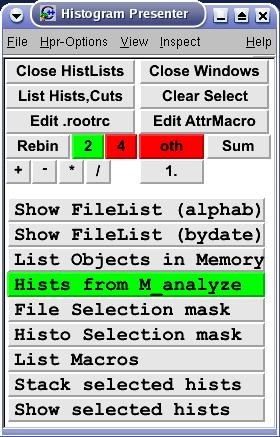
\includegraphics[width=\linewidth]{HistPresentGUI}}
\caption{\texttt{HistPresent}}
\label{HistPresentConnect}
\end{figure}
\end{minipage}\qquad\qquad
\begin{minipage}[t]{.4\linewidth}
\begin{figure}[H]
\centerline{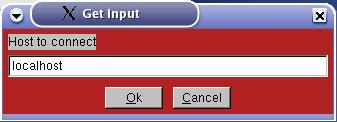
\includegraphics[width=\linewidth]{HistPresentConnectToHost}}
\end{figure}
\begin{figure}[H]
\centerline{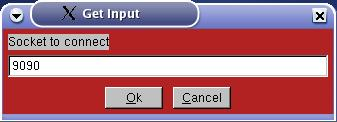
\includegraphics[width=\linewidth]{HistPresentConnectToSocket}}
\caption{Connect to \texttt{M\_analyze}}
\end{figure}
\end{minipage}
\end{center}

\subsection{How to reset MBS manually}\label{ResetMBSManually}\vspace{3mm}

In case the \blue{Clear MBS} button of \texttt{C\_analyze} doesn't work as expected you have
to reset \texttt{MBS} manually. (Open a new \texttt{xterm}, then) type\\

\hspace*{.2\linewidth}\yellow{rsh ppc-0} to login to the ppc.\\

Then change directory to the current experiment:\\

\hspace*{.2\linewidth}\yellow{cd <my\_working\_directory>/ppc}
\hspace{1cm}(example: \yellow{cd cern-040719/ppc})

Then type

\hspace*{.2\linewidth}\yellow{resmbs}\\

This should kill all MBS processes (the ones starting with \yellow{m\_} in the name when doing \yellow{ps ax}).\\

If there is some error message during \texttt{resmbs} ("device busy" or similar) you should do a \yellow{ps ax}
and look for the line containing the \texttt{m\_prompt} process:\\

\hspace{2cm}\texttt{53    1   53  18  168     8   68      0.05       miniball W /mbs/deve/bin\_RIO2/m\_prompt}\\

Pick the first number from this line then and kill this process by typing\\

\hspace*{.2\linewidth}\yellow{kill <proc\_no>}
\hspace{1cm}(this example: \yellow{kill 53})\\

Type \yellow{logout} to leave the ppc session.

\subsection{How to generate and to compile code}\label{GenerateAndCompileCode}\vspace{3mm}

To update the DGF cluster settings you have to edit files
\begin{center}
\begin{tabular}{ll}		
\yellow{cluster.def}		&	settings for \textbf{active} clusters\\
\yellow{cluster-void.def}	&	settings for clusters which are currently \textbf{inactive} but have DGF modules assigned\\
\yellow{other-dgfs.def}		&	settings for other DGF modules such as time stamper, beam dump detector, etc.\\
\end{tabular}
\end{center}
The file format is adopted from Nigel Warr's Miniball Configuration sheet. See \ref{ClusterDef} for a description.\\

\redt{CAVEAT:}
Make sure that \textbf{all existing} DGF modules are defined in these files. Otherwise any uninitialized DGF will spoil its CAMAC crate!\\

To generate your code from the config file simply type\\

\hspace*{.2\linewidth}\yellow{./Config.C} \\

This will generate all code files needed for the experiment (fig. \ref{ConfigStep}). Existing files will be overwritten.\\

To compile the \texttt{ROOT} part of the code (running on your desktop under \texttt{Linux}) type\\

\hspace*{.2\linewidth}\yellow{make -f DgfAnalyze.mk clean all}\\

This will compile and link program \texttt{M\_analyze} which is then used by the control GUI \texttt{C\_analyze}.\\
This step has to be repeated whenever you made changes in the configuration or in the user part of your code (code files residing
in the \texttt{udef} subdirectory).\\

To compile the readout part of your code (running under \texttt{MBS}) call \yellow{C\_analyze}, then click on\\

\hspace*{.2\linewidth}\blue{Mbs Control}$\rightarrow$\blue{Compile readout function} (fig. \ref{CanalyzeCompileReadout})\\

Alternatively you may compile the readout code in the ppc directly:\\

\hspace*{.2\linewidth}\yellow{rsh ppc-0}\\
\hspace*{.2\linewidth}\yellow{cd <my\_working\_directory>/ppc}\\
\hspace*{.2\linewidth}\yellow{make -f DgfReadout.mk clean all}\\
\hspace*{.2\linewidth}\yellow{logout}\\

This will produce \texttt{MBS} task \texttt{m\_read\_meb} in subdirectory \texttt{ppc}.\\
Repeat this step whenever the hardware config has changed (e.g. number and position of \texttt{VME} and \texttt{CAMAC} modules). 

\begin{figure}[H]
\centerline{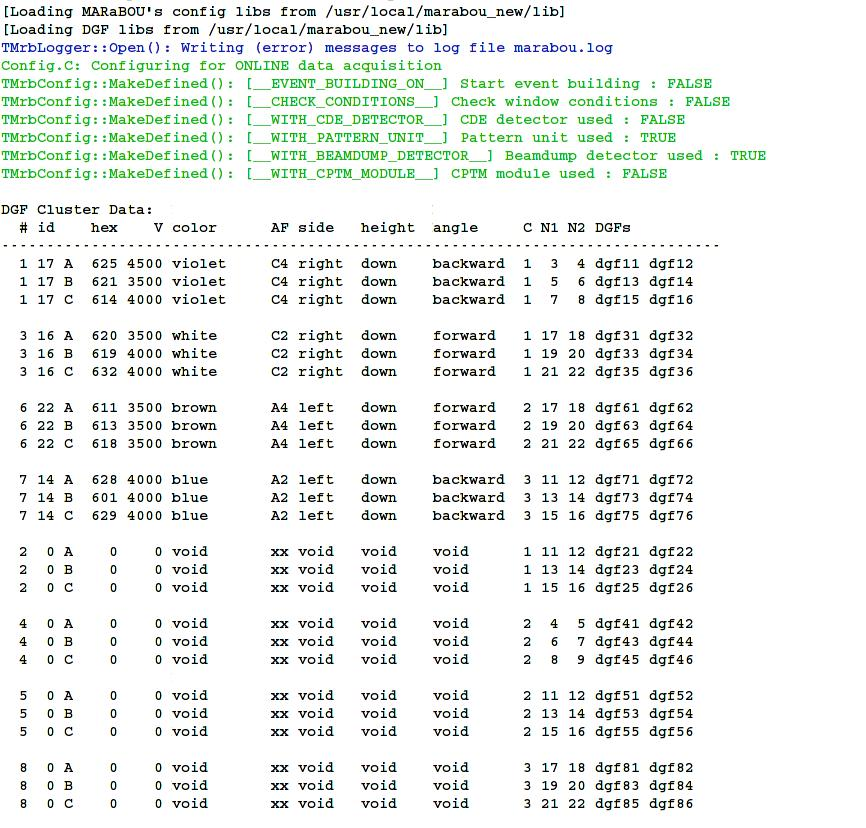
\includegraphics[width=\linewidth]{ConfigStep1}}
\centerline{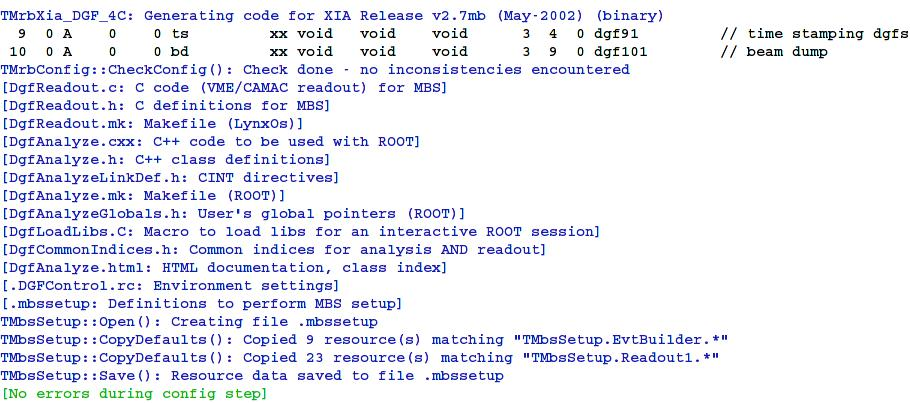
\includegraphics[width=\linewidth]{ConfigStep2}}
\caption{\texttt{Config.C}: generating code files}
\label{ConfigStep}
\end{figure}

\begin{figure}[H]
\centerline{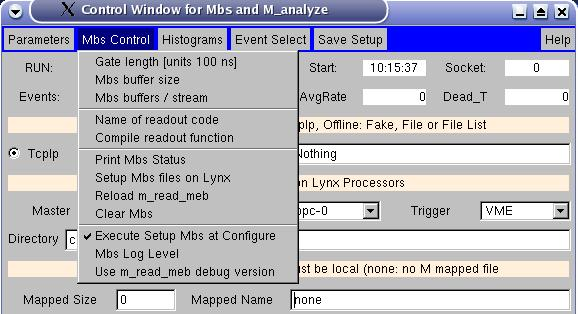
\includegraphics[width=\linewidth]{C_analyzeCompileReadout}}
\caption{\texttt{C\_analyze}: how to compile readout task}
\label{CanalyzeCompileReadout}
\end{figure}
\newpage
\subsection{How to establish a directory for an offline session}\label{OfflineSession}\vspace{3mm}

In an online run only a few diagnostic tests may be performed beside data taking.
To evaluate data one has to establish an offline session in parallel.\\

To start an offline session you first have to create directories and subdirectories and to copy and link files which are identically
used in online and offline sessions. script \yellow{mkoffl} will do the job:

\hspace*{.2\linewidth}\yellow{cd /d1/miniball}\\
\hspace*{.2\linewidth}\yellow{mkoffl <online\_dir>}\\

It creates an offline directory \texttt{<online\_dir>-offline}.
This naming convention will later on be used by script \yellow{Config.C} to distinguish between online and offline.\\

\yellow{mkoffl} will do the following:

\begin{center}
\begin{itemize}
\setlength{\rightmargin}{1em}%
\setlength{\leftmargin}{2em}%
\setlength{\itemsep}{0pt}%
\setlength{\parskip}{1mm}%
\setlength{\partopsep}{0pt}%
\setlength{\parsep}{0pt}%
\setlength{\topsep}{0pt}%
\item	create subdirectories \texttt{<online\_dir>-offline/udef} and \texttt{<online\_dir>-offline/config}
\item	copy \texttt{<online\_dir>/.rootrc}
\item	copy contents of subdir \texttt{<online\_dir>/config}
\item	copy "ifdefs" in \texttt{<online\_dir>/SetCppIfdefs.C}
\item	copy calibration files \texttt{<online\_dir>/*.cal}
\item	link config file \texttt{<online\_dir>/Config.C}
\end{itemize}
\end{center}

Now one has to create/modify files to meet offline requirements:
\begin{center}
\begin{itemize}
\setlength{\rightmargin}{1em}%
\setlength{\leftmargin}{2em}%
\setlength{\itemsep}{0pt}%
\setlength{\parskip}{1mm}%
\setlength{\partopsep}{0pt}%
\setlength{\parsep}{0pt}%
\setlength{\topsep}{0pt}%
\item	modify entries in \yellow{SetCppIfdefs.C} (enable event building and window check for example)
\item	book additional histograms in file \yellow{BookHistogramsOffline.C}
\item	define window settings in \yellow{DefineVarsAndWdws.C}
\item	place your analysis code in subdirectory \boldt{udef}: \yellow{udef/Analyze.cxx + .h}
\end{itemize}
\end{center}

You should then be able to perform the config step and to compile and link your code (see \ref{GenerateAndCompileCode}):
\begin{center}
\begin{blueboxed}{.75\linewidth}
\verb+	./Config.C+\\
\verb+	make -f DgfAnalyze.mk clean all+
\end{blueboxed}
\end{center}

Now start \yellow{C\_analyze} and attach to the \texttt{.med} file which is being actually produced in the online directory.
You may thus perform a "quasi-online" run in parallel to the real online data acquisition.
\newpage
\subsection{How to start a new session in a new directory}\label{CreateNewDir}\vspace{3mm}

To start a new experiment in a new working directory go one level up:\\

\hspace*{.2\linewidth}\yellow{cd /d1/miniball}\\

Then type\\

\hspace*{.2\linewidth}\yellow{mknew <old\_dir> <new\_dir>}\\

where \texttt{<old\_dir>} is the directory you worked before, \texttt{<new\_dir>} is the one you want to start a new experiment in.\\

\yellow{mknew} will do the following:

\begin{center}
\begin{itemize}
\setlength{\rightmargin}{1em}%
\setlength{\leftmargin}{2em}%
\setlength{\itemsep}{0pt}%
\setlength{\parskip}{1mm}%
\setlength{\partopsep}{0pt}%
\setlength{\parsep}{0pt}%
\setlength{\topsep}{0pt}%
\item	copy \texttt{<old\_dir>/*.C} to \texttt{<new\_dir>}
\item	copy \texttt{<old\_dir>/.rootrc} to \texttt{<new\_dir>}
\item	copy \texttt{<old\_dir>/*.def} to \texttt{<new\_dir>}
\item	copy subdirectories \texttt{<old\_dir>/udef} and \texttt{<old\_dir>/config} to \texttt{<new\_dir>}
\item	create subdirectory \texttt{<new\_dir>/ppc}
\item	perform a config step calling \texttt{<new\_dir>/Config.C} (2x \texttt{:-(})
\item	compile and link program \texttt{M\_analyze} to be used by \texttt{C\_analyze}
\end{itemize}
\end{center}

You should then be able to run \yellow{C\_analyze}. Follow instructions in \ref{SetupListmodeRun} to setup your experiment properly.
Don't forget to re-compile the \texttt{MBS} readout task before starting data acquisition (\ref{GenerateAndCompileCode}).
\newpage
\subsection{How to produce an ascii dump of \texttt{.med} data}\label{ProduceAsciiDump}\vspace{3mm}

There is a tool called \yellow{mbs2asc} which may be used to dump \texttt{.med} data to ascii for debugging purposes.\\

{\scriptsize
\begin{yellowboxed}{\linewidth}
\verb+Usage: mbs2asc [-r <rcFile>] [-n <maxEvents>] [-t <rdoTrig>] [-f <dgfFmt>]+\\
\verb+                                               [-d <sevtType>] [-v] <mbsFile>+\\
\verb+ +\\
\verb+mbsFile        raw data file (extension .lmd or .med)+\\
\verb+ +\\
\verb+-r <rcFile>    use indices and defs from <rcFile> (default: no defs)+\\
\verb+-n <maxEvents> process <maxEvents> only (default: end of file)+\\
\verb+-t <rdoTrig>   readout trigger is <trigger> (default: 1)+\\
\verb+               (there may be more than one option "-t" in case of multiple triggers)+\\
\verb+-f <dgfFmt>    use DGF-4C format descriptor <dgfFmt> in case of format errors+\\
\verb+-d <sevtType>  raw data file contains subevent dumps rather than original mbs data (extension .dmp)+\\
\verb+               <sevtType> = "dgf" or "caen" (default: none)+\\
\verb+-v             turn on verbose mode: output hex dump in addition to other data+
\end{yellowboxed}}\\

For example, command\\

\centerline{\blue{mbs2asc -r .DGFControl.rc -n 10 -v run140.med | less}}\vspace{3mm}

will produce output\\

{\scriptsize
\begin{yellowboxed}{\linewidth}
\verb+# Program                    : mbs2asc+\\
\verb+# Arguments                  : -r .DGFControl.rc -n 10 -v run140.med+\\
\verb+# Input                      : run140.med+\\
\verb+# Indices & defs             : .DGFControl.rc+\\
\verb+# Event trigger(s)           : 1+\\
\verb+# Max number of events       : 10+\\
\verb+# Verbose mode               : on+\\
\verb+ ... +\\
\verb+MBS EVT    10     1   14 	1 1594049             # start acquisition (trigger #14)+\\
\verb+MBS EVT    10     1    1 	2 1594050             # readout (trigger #1)+\\
\verb+MBS SEVT 9000     1  999                        # subevent "Time stamp"+\\
\verb+MBS SEVT   10    23  	 2                        # subevent "clu2"+\\
\verb+DGF BUF   36      7  257  0       0   65167   65167 # 0024 0007 1101 0000 0000 fe8f # module "dgf21"+\\
\verb+DGF EVT    7                      1   17443   82979 # 0007 0001 4423+\\
\verb+DGF CHN    0   2663                   17468   83004 # 0008 443c 0a67 1618 1af0 0000 0000 0000+\\
\verb+DGF CHN    1      0                   17468   83004 # 0008 443c 0000 0000 0000 ffd5 000b 0000+\\
\verb+DGF CHN    2      0                   17468   83004 # 0008 443c 0000 0daf 0000 002c 0003 0000+\\
\verb+DGF BUF   45      8  257  0       0   65167   65167 # 002d 0008 1101 0000 0000 fe8f # module "dgf22"+\\
\verb+DGF EVT   15                      1   17443   82979 # 000f 0001 4423+\\
\verb+DGF CHN    0   2541                   17468   83004 # 0008 443c 09ed 0000 0000 ff70 0021 0000+\\
\verb+DGF CHN    1      0                   17468   83004 # 0008 443c 0000 0c80 0000 ffe8 0006 0000+\\
\verb+DGF CHN    2      0                   17468   83004 # 0008 443c 0000 0000 0000 0015 001d 0000+\\
\verb+DGF CHN    3      0                   17468   83004 # 0008 443c 0000 0000 0000 ffee 0018 0000+\\
\verb+DGF BUF   36      9  257  0   0       65166   65166 # 0024 0009 1101 0000 0000 fe8e # module "dgf23"+\\
\verb+DGF EVT    7                  3        5923  202531 # 0007 0003 1723+\\
\verb+DGF CHN    0  12127                    5947  202555 # 0008 173b 2f5f 1770 1e57 0000 0000 0000+\\
\verb+DGF CHN    1      0                    5947  202555 # 0008 173b 0000 0000 0000 ffe1 0010 0000+\\
\verb+DGF CHN    2      0                    5947  202555 # 0008 173b 0000 0000 0000 ffd7 0016 0000+\\
\end{yellowboxed}}

\newpage
\section{Set up and control XIA DGF-4C modules}\vspace{3mm}

\texttt{DGFControl} is a program to set up the DGFmodules for the DAQ.
It is NOT necessary to restore the \texttt{DGF} parameter settings for each run.
Only if the \texttt{CAMAC} crates have been switched off or the \texttt{DGF} modules have been booted
they have lost their parameters.
Fortunately the settings have been saved and can be restored from file
(don't forget to save your settings after a change!).\\

\redt{CAVEAT:}
Connecting to \texttt{DGF} modules via \texttt{DGFControl} may disturb a running data acquisition.
Be sure that no daq is running or that you pressed \texttt{Stop} or \texttt{Pause} in the \texttt{C\_analyze} GUI to stop it.\\


Open a new \texttt{xterm} window. Then type\\

\hspace*{.2\linewidth}\yellow{DGFControl}\\

The main (\texttt{system}) tab should then show up at your screen (fig. \ref{DgfControlSystemTab}.\\

\hspace*{.2\linewidth}press \blue{Restart ESONE} to (re-)start the \texttt{CAMAC} server\\

\hspace*{.2\linewidth}press \blue{Reload DGFs} to download the volatile DSP and FPGA code\\

(this has to be done whenever the \texttt{CAMAC} crates has been switched off)\\

\hspace*{.2\linewidth}press \blue{Connect} \\

Then open the \texttt{Restore} tab and reload the appropriate parameter settings.\\

Visit shortly the \texttt{Files} and \texttt{Modules} tabs
   to check if the right DSP/FPGA code has been downloaded and the DSP parameters
   are correct. If the file names differ from what you expect you'll
   have to set the proper values in your \texttt{.rootrc} file and to start over.
   If the shaping times for the DGFs are not 6.8 us peaking and 2 us gap time,
   you probably forgot to restore parameters.\\

The list below describes what the different tabs in \texttt{DGFControl} are meant for.\\
\begin{center}
\begin{itemize}
\setlength{\rightmargin}{1em}%
\setlength{\leftmargin}{2em}%
\setlength{\itemsep}{0pt}%
\setlength{\parskip}{1mm}%
\setlength{\partopsep}{0pt}%
\setlength{\parsep}{0pt}%
\setlength{\topsep}{0pt}%
\item	\blue{System} (fig. \ref{DgfControlSystemTab})\\
	Restart \texttt{ESONE/CAMAC} server, reload (= boot) dgf modules,
	connect to modules if server is still running
\item	\blue{Modules} (fig. \ref{DgfControlModulesTab})\\
	Control and change modules settings, one sheet per module/channel
\item	\blue{Params}\\
	Show a given param for all modules. You may change single params or set a param for all modules selected.
\item	\blue{Traces}\\
	Accumulate triggered traces for all modules activated (one trace per module/channel).
	Data will be written to a \texttt{ROOT} file \texttt{trace.root},
	and may afterwards be looked at via \texttt{HistPresent}.
\item	\blue{Untrig Traces}\\
	Collect untriggered traces for all modules selected. Results are stored in file \texttt{untrigTrace.root}
\item	\blue{Offsets}\\
	Start a "\texttt{ramping dacs}" task and adjust offsets. Untriggered traces should then have their baselines at
	4 times the offset value.
\item	\blue{MCA} (fig. \ref{DgfControlMcaTab})\\
	Start a \texttt{MCA} run. At end of accumulation histograms will be dumped on the ppc side, then converted to
	\texttt{ROOT} format and stored in file \texttt{mca.root}. To be looked at by \texttt{HistPresent}.
\item	\blue{TauDisplay}\\
	Accumulate a number of triggered traces for selected module. Results will be displayed in a separate canvas.
\item	\blue{Misc}\\
	Miscellaneous: Set/clear GFLT, set COINCWAIT
\item	\blue{Save}\\
	Save dgf parameters to disk. Should be done on major changes to the dgf parameters.
\item	\blue{Restore}\\
	Restore dgf parameters from disk
\item	\blue{Copy}\\
	Copy certain parameters from one module/channel to others
\item	\blue{Files}\\
	A list of files currently used
\item	\blue{CPTM} (fig. \ref{DgfControlCptmTab})\\
	A panel to control the "Clock and Programmable Trigger" module (CPTM, Univ Cologne)
\end{itemize}
\end{center}
\begin{figure}[H]
\centerline{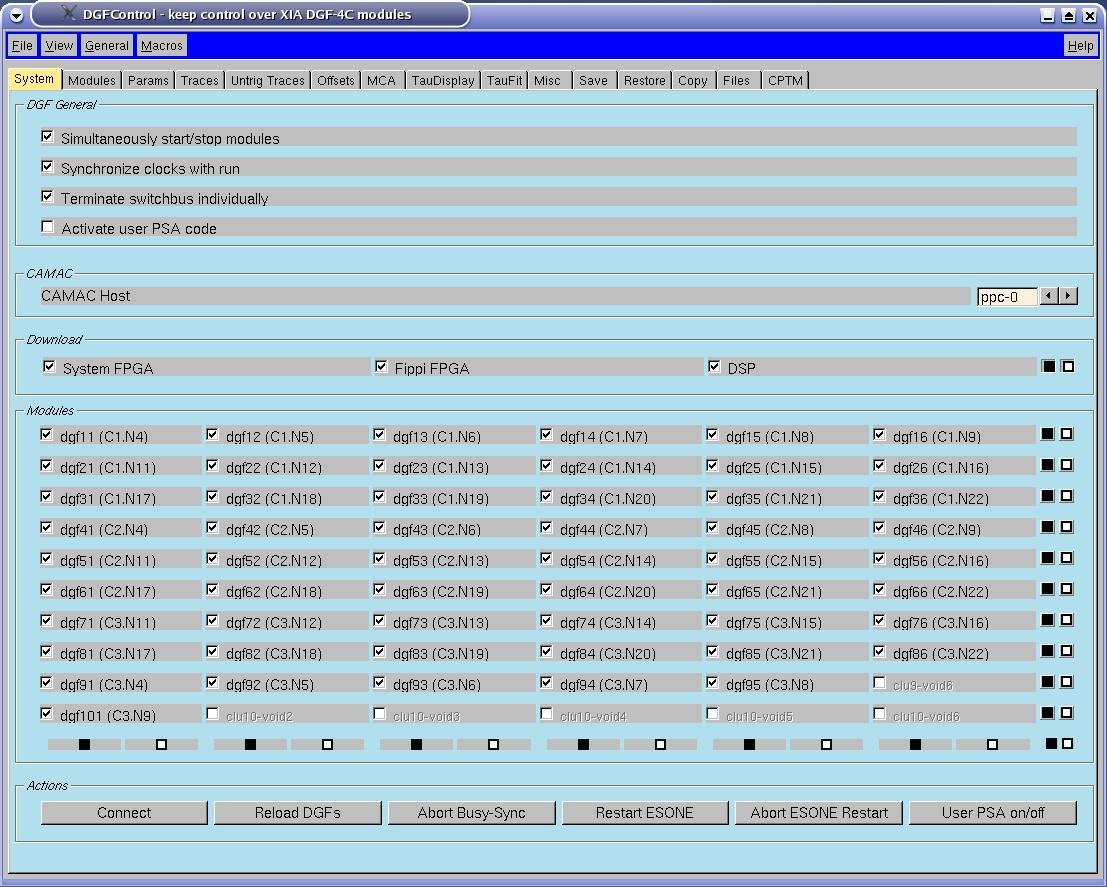
\includegraphics[width=1.2\linewidth]{DgfControlSystemTab}}
\caption{\texttt{DgfControl}: how to set up and control \texttt{XIA DGF-4C} modules}
\label{DgfControlSystemTab}
\end{figure}
\newpage
\begin{figure}[H]
\centerline{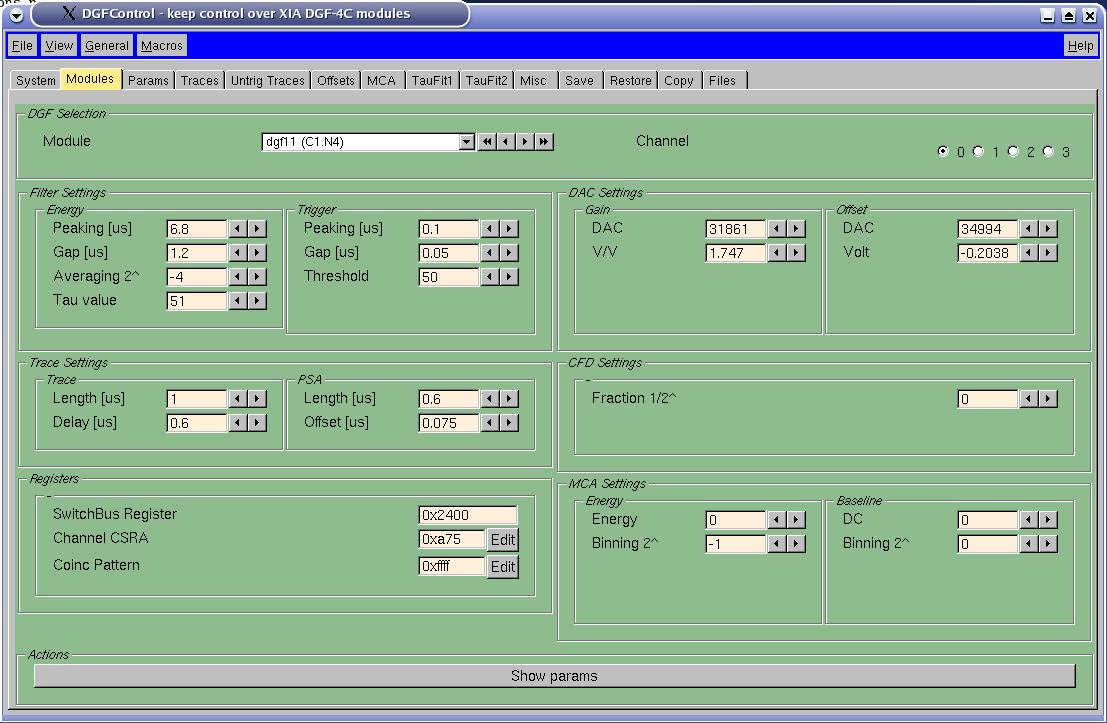
\includegraphics[width=1.2\linewidth]{DgfControlModulesTab}}
\caption{\texttt{DgfControl}: display parameter settings of \texttt{XIA DGF-4C} modules}
\label{DgfControlModulesTab}
\end{figure}
\begin{figure}[H]
\centerline{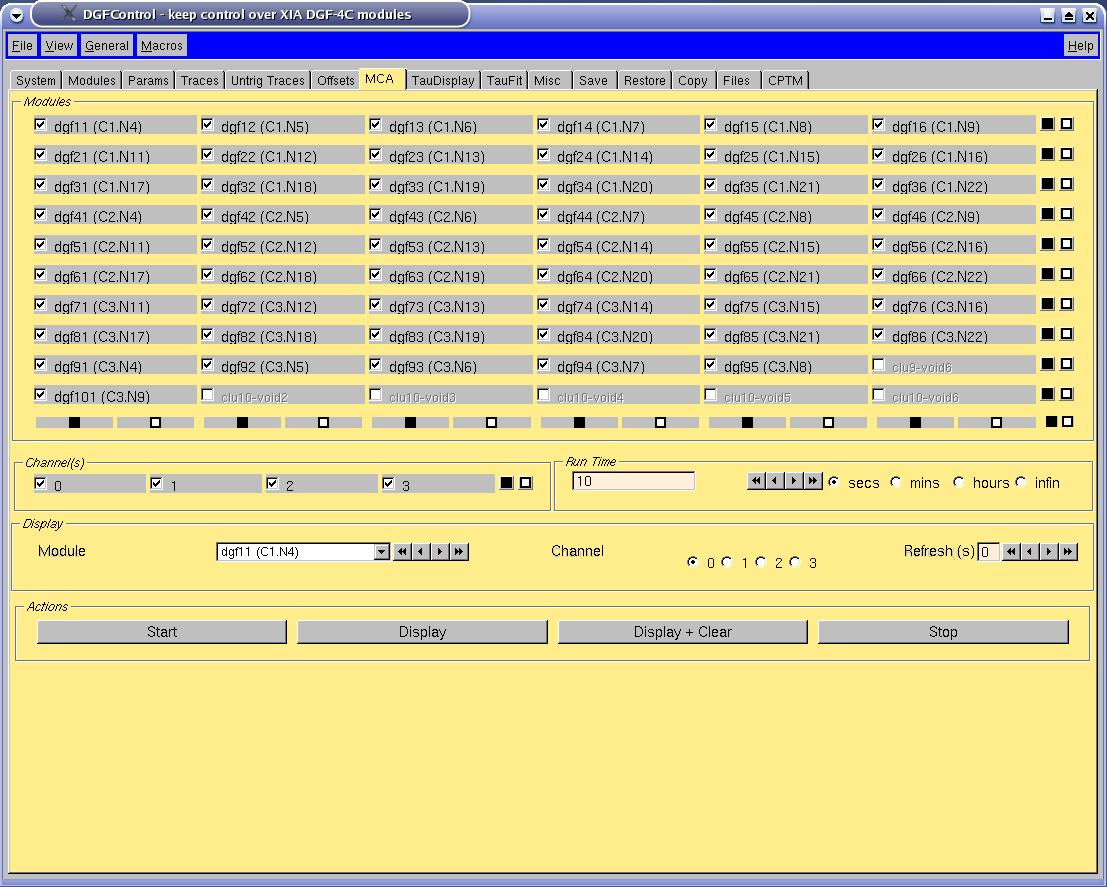
\includegraphics[width=\linewidth]{DgfControlMcaTab}}
\caption{\texttt{DgfControl}: start a \texttt{MCA} accumation}
\label{DgfControlMcaTab}
\end{figure}
\begin{figure}[H]
\centerline{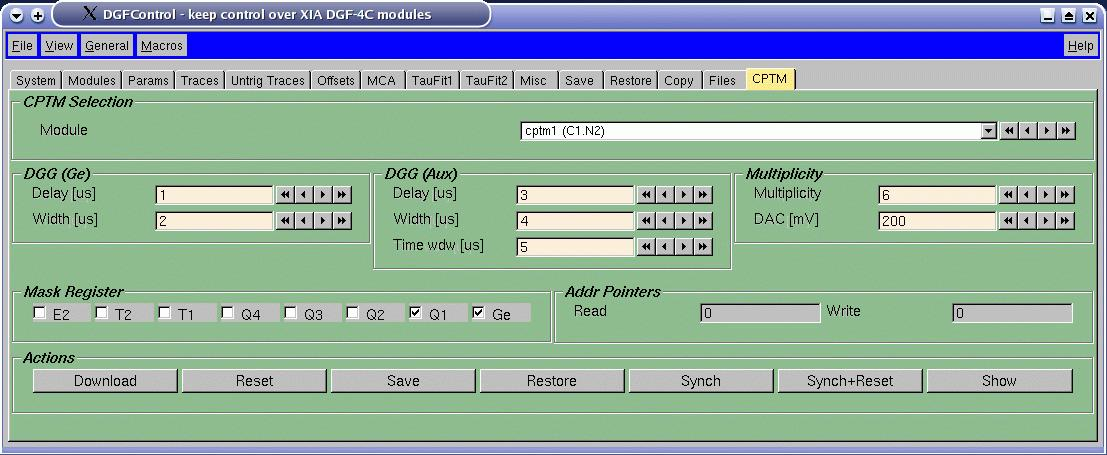
\includegraphics[width=\linewidth]{DGFCptmPanel}}
\caption{\texttt{DgfControl}: how to control a \texttt{CPTM} module}
\label{DgfControlCptmTab}
\end{figure}
\newpage
\section{How to perform an energy calibration}\vspace{3mm}

Oliver's program for energy calibration has now been modified to output data compatible with \MARaBOU{}. So a conversion of the
calibration data thru \texttt{olli2rudi} is no longer necessary.\\

To do an energy calibration (gamma or particle) call the \texttt{MacroBrowser}:\\

\hspace*{.2\linewidth}\yellow{MacroBrowser}\\

A menu will then pop up showing several \texttt{ROOT} macros. Choose \blue{MBcal.C} from this list.\\

You'll get a form (fig. \ref{MBcal}) to specify which type of calibration on which histograms you want to do:
\begin{center}
\begin{itemize}
\setlength{\rightmargin}{1em}%
\setlength{\leftmargin}{2em}%
\setlength{\itemsep}{0pt}%
\setlength{\parskip}{1mm}%
\setlength{\partopsep}{0pt}%
\setlength{\parsep}{0pt}%
\setlength{\topsep}{0pt}%
\item	\blue{Calibration}\\
	Choose \texttt{Co60} or \texttt{Eu152} for gammas, \texttt{TripleAlpha} for particles
\item	\blue{Histo file / first histo}\\
	Click on the folder button and choose the \texttt{ROOT} file containing your calibration spectra.
	Choose histogram to start with.
\item	\blue{Histo file / last histo}\\
	You have to select the \textbf{same} \texttt{ROOT} file as above. Choose the histogram to end with.
\item	\blue{Calibration output file}\\
	where calibration data should be stored.\\
	This name should correspond to entries\\
	\hspace*{3cm}\yellow{TMrbAnalyze.CalibrationFile.DGF} (gamma) or\\
	\hspace*{3cm}\yellow{TMrbAnalyze.CalibrationFile.Caen} (particle)\\
	in your \texttt{.rootrc}.
	The extension has to be \texttt{.cal}.
\item	\blue{Results file}\\
	where Oliver writes detailed calibration results
\item	\blue{Precalibration file}\\
	To get an \texttt{Eu152} calibration you have to preform a \texttt{Co60} calibration step first.
	The name of the \texttt{Co60} calibration file has to be given here.
\item	\blue{Verbose output}
\item	\blue{Sigma for PeakFind} choose at least \texttt{5}
\item	\blue{Relative percentage for PeakFind} \texttt{5}
\item	\blue{Peaks to be fitted} \texttt{No}
\item	\blue{Zero bins in front} \texttt{100}
\end{itemize}
\end{center}
Press \blue{Execute} to start the calibration.
Resulting calibration files will be read upon restart of your data acquisition (i.e. on next \texttt{Start} in \texttt{C\_analyze}).
For a description of the file format see \ref{MBcalFileFormat}
\newpage
\begin{figure}[H]
\centerline{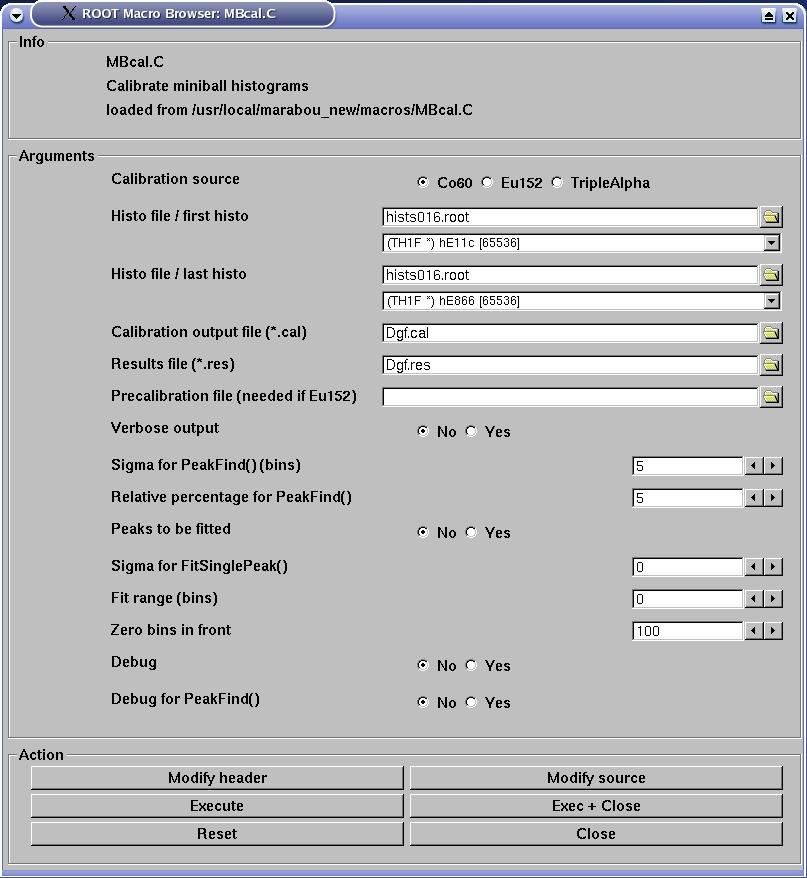
\includegraphics[width=\linewidth]{MBcalForm}}
\caption{\texttt{MBcal.C}: how to do an energy calibration}
\label{MBcal}
\end{figure}
\newpage
\section{How to do a Doppler correction}\vspace{3mm}
\subsection{Doppler correction modes}\vspace{3mm}

To do a Doppler correction you have to create a file containing the correction coefficients for each
histogram. A Doppler correction may be defined in three different ways.
\begin{center}
\begin{itemize}
\setlength{\rightmargin}{1em}%
\setlength{\leftmargin}{2em}%
\setlength{\itemsep}{0pt}%
\setlength{\parskip}{1mm}%
\setlength{\partopsep}{0pt}%
\setlength{\parsep}{0pt}%
\setlength{\topsep}{0pt}%
\item	\textbf{Using a constant factor}\\
	You may have taken the Doppler shift from a fit to your histograms. The dcorr file then has one entry per histogram
	containing this factor.
\item	\textbf{Using a fixed geometry}\\
	If the particle is going in $0^\circ$ forward direction the Doppler correction is given by the particle
	verlocity and the detection angle for cores and segments, respectively.
	Add one entry per histogram to the dcorr file containing this
	angle (degrees or radians).
\item	\textbf{Using a geometry depending on particle angle}\\
	You have to perform kinematic calculations to get velocity and angle for each particle
	independently. The dcorr file should then contain the detection angles with respect to $0^\circ$ for each core and segment.
\end{itemize}
\end{center}

Add an entry\\
	\hspace*{3cm}\yellow{TMrbAnalyze.DCorrFile.DGF:	<dcorr file>}\\
	
to your \texttt{.rootrc}. The file extension has to be \texttt{.dcorr}.
Doppler correction data will then be read from this file upon restart of your data acquisition
(i.e. on next \texttt{Start} in \texttt{C\_analyze}).\\

For a description of the file format see \ref{DCorrFileFormat}.
\newpage
\section{Appendix}\vspace{3mm}
\subsection{Scripts}\vspace{3mm}

There are some scripts that should be run to monitor that everything
works as expected.  The purpose and how to start a certain script is
explained below:\\

\yellow{scaler.sh}\\

This script displays the trigger scalers. See \ref{ScalerData}.
It shows the rate with which some detectors or the DAQ are triggering.\\
Stop it by pressing Ctrl-C. \\

\yellow{dgfscaler.sh}\\

This script displays the internal DGF scalers (\ref{ScalerData}).\\
Stop it by pressing Ctrl-C. \\

\yellow{ppac.sh}  \redt{[obsolete]}\\

Script to display the location of the beam in X and Y direction as measured
with the PPAC.\\
No longer used, call \yellow{ppac.C} instead (\ref{PPAC}).\\

\yellow{start\_rate\_monitor.sh} \redt{now WITHOUT leading "./"!} \redt{[obsolete]}\\

Should be started once and should run all the time.
It produces the files needed by the \texttt{plot\_rate2.gp} script (see below).
In case the rate plots are not updating even though the DAQ is running it
might be that this script needs to be started again.\\
Script exits by itself.\\
Script is obsolete now -- call \yellow{rateMon.C} instead (\ref{RateMon}).\\

\yellow{plot\_rate2.gp} \redt{now WITHOUT leading "./"!} \redt{[obsolete]}\\

\texttt{Gnuplot} script that displays the 444 keV rate (bottom) and the beam
dump rate (top) for 1, 5, 17, and 34 second averages.\\
Stop it by pressing Ctrl-C. \\ 
Script is obsolete now -- call \yellow{rateMon.C} instead (\ref{RateMon}).\\

\yellow{monitor\_rates.sh \textit{threshold}} \redt{now WITHOUT leading "./"!} \redt{[obsolete]}\\

The keyboard bell rings and the screen flashes if the 17 second average
444 keV rate drops below the threshold given.  In that case most
likely the beam is gone and it should be checked if everything is
still running.\\
Stop it by pressing Ctrl-C.\\
Script is obsolete now -- call \yellow{rateMon.C} instead (\ref{RateMon}).\\

\yellow{CDThresPed2C <CDThres.ped >CDThres.C} \redt{now WITHOUT leading "./"!}\\

Script used by \texttt{Config.C} during config step to convert pedestal file \texttt{CDThres.ped} to \MARaBOU{} commands in
\texttt{CDThres.C}. Edit \texttt{CDThres.ped} according to your needs first.\\


\yellow{nigel2cluster \textit{psFile} \textit{cluFile}}\\

Script to convert Nigel's miniball config sheet from PostScript to ascii. \texttt{cluFile} is expected to have extension \texttt{.def}.

\newpage
\subsection{Files related to Config.C}
\subsubsection{Input files}\vspace{3mm}

To run a configuration step by executing \yellow{./Config.C} successfully several input files have to be present
\begin{itemize}
\setlength{\rightmargin}{1em}%
\setlength{\leftmargin}{2em}%
\setlength{\itemsep}{0pt}%
\setlength{\parskip}{1mm}%
\setlength{\partopsep}{0pt}%
\setlength{\parsep}{0pt}%
\setlength{\topsep}{0pt}%
\item	\yellow{in your working directory:}
	\begin{itemize}
	\setlength{\rightmargin}{1em}%
	\setlength{\leftmargin}{2em}%
	\setlength{\itemsep}{0pt}%
	\setlength{\parskip}{1mm}%
	\setlength{\partopsep}{0pt}%
	\setlength{\parsep}{0pt}%
	\setlength{\topsep}{0pt}%
	\item	\yellow{\$HOME/.rootrc} and \yellow{.rootrc}\\
		contain \texttt{ROOT} resource definitions to control the config step\\
		define paths to other inputs like templates, macros, etc.
	\item	\yellow{cluster.def}, \yellow{cluster-void.def}, \yellow{other-dgfs.def}\\
		cluster definitions for active clusters, unsed clusters, and other dgf modules, resp.\\
		See \ref{ClusterDef} for file format.
	\item	\yellow{SetCppIfdefs.C}
		defines \texttt{\#ifdef} settings for the cpp preprocessor:
		\begin{itemize}
		\setlength{\rightmargin}{1em}%
		\setlength{\leftmargin}{2em}%
		\setlength{\itemsep}{0pt}%
		\setlength{\parskip}{1mm}%
		\setlength{\partopsep}{0pt}%
		\setlength{\parsep}{0pt}%
		\setlength{\topsep}{0pt}%
		\item	Turn on event building (\texttt{online:off})
		\item	Perform a window check for each event (\texttt{online:no})
		\item	Use the CDE detector 
		\item	Use a pattern unit
		\item	Used the beamdump detector
		\end{itemize}
	\item	\yellow{BookHistograms.C}
		contains user's histogram definitions. Executed as part of \texttt{Config.C}.\\
		It is recommended to put any histogram defs in this file to increase readability.
	\item	\yellow{BookHistogramsOffline.C} (offline only)\\
		contains additional histogram defs for an \texttt{offline} session
	\item	\yellow{DefineVarsAndWdws.C} (offline only)\\
		defines windows and cuts for an \texttt{offline} session
	\item	\yellow{cluster.def} and \yellow{cluster-void.def}\\
		both define the cluster configuration to be used by \texttt{Config.C}. \texttt{cluster.def} contains active clusters as
		given by Nigel's configuration sheet, whereas \texttt{cluster-void.def} contains crate as well
		as station numbers for dgf modules
		currently unused (but present). Use script \texttt{nigel2cluster} to convert Nigel's PostScript
		file to \texttt{cluster.def}. 
	\item	\yellow{other-dgfs.def}\\
		defines crate and station numbers for other dgfs such as time stamper and beamdump. Will also be read by \texttt{Config.C}.
	\end{itemize}
\item	\yellow{in subdirectory config} (has to be part of resource \texttt{.rootrc:TMrbConfig.MacroPath})
	\begin{itemize}
	\setlength{\rightmargin}{1em}%
	\setlength{\leftmargin}{2em}%
	\setlength{\itemsep}{0pt}%
	\setlength{\parskip}{1mm}%
	\setlength{\partopsep}{0pt}%
	\setlength{\parsep}{0pt}%
	\setlength{\topsep}{0pt}%
	\item	\yellow{UserMacro.C}\\
		contains user's code generation macros either as a replacement of or an extension to standard macros
		provided by \MARaBOU{} (change only if you are an expert).
	\item	several special templates used by \yellow{UserMacro.C} (don't touch either)
	\end{itemize}
\item	\yellow{in subdirectory udef}
	\begin{itemize}
	\setlength{\rightmargin}{1em}%
	\setlength{\leftmargin}{2em}%
	\setlength{\itemsep}{0pt}%
	\setlength{\parskip}{1mm}%
	\setlength{\partopsep}{0pt}%
	\setlength{\parsep}{0pt}%
	\setlength{\topsep}{0pt}%
	\item	\yellow{BuildEvent.cxx/.h}
		how to build events from user's raw data
	\item	\yellow{Analyze.cxx/.h}
		user's analysis event by event
	\item	\yellow{TUsrHitEvent.cxx/.h}
		intermediate event structure during event building
	\item	\yellow{Exp.h}
		final event structure after event building
	\item	\yellow{HelpFunct.h}
		some helper functions
	\item	\yellow{Winfo.h}
		window definitions
	\end{itemize}
\item	\yellow{in the directory pointed to by resource \texttt{.rootrc:TMrbConfig.TemplatePath}}
	\begin{itemize}
	\setlength{\rightmargin}{1em}%
	\setlength{\leftmargin}{2em}%
	\setlength{\itemsep}{0pt}%
	\setlength{\parskip}{1mm}%
	\setlength{\partopsep}{0pt}%
	\setlength{\parsep}{0pt}%
	\setlength{\topsep}{0pt}%
	\item	template files to generate code for readout and analysis, respectively
	\item	templates files to generate files needed for MBS setup
	\end{itemize}
\end{itemize}

\subsubsection{Output files}\vspace{3mm}

Any output created by \texttt{Config.C} is written to the user's working directory.
File names will be derived from the name of the config object in user's \texttt{Config.C}. If this object is
named \blue{dgf} for example, any file name created by \texttt{Config.C} will start with the prefix \blue{Dgf\dots{}}.
Any file starting with this prefix may be deleted without consequence - it can be re-generated by simply calling \yellow{./Config.C}.

\begin{itemize}
\setlength{\rightmargin}{1em}%
\setlength{\leftmargin}{2em}%
\setlength{\itemsep}{0pt}%
\setlength{\parskip}{1mm}%
\setlength{\partopsep}{0pt}%
\setlength{\parsep}{0pt}%
\setlength{\topsep}{0pt}%
\item	\yellow{.DgfConfig.rc}\\
	any names, counters, indices etc. created during the config step.\\
	Written using \texttt{ROOT}'s resource format.\\
	This file may be input by other service programs (such as \texttt{DGFControl}) 
\item	\yellow{DgfCommonIndices.h}\\
	indices, serial numbers etc. to be used by both readout and analysis programs.
\item	\yellow{DgfReadout.c/.h}\\
	user's readout function loaded as part of \texttt{MBS} task \texttt{m\_read\_meb}.
\item	\yellow{DgfReadout.mk}\\
	Makefile to compile and link \texttt{MBS} task \texttt{m\_read\_meb} on ppc.
\item	\yellow{DgfAnalyze.cxx/.h}\\
	user's code generated automatically. Makes up main part of \texttt{M\_analyze}.
\item	\yellow{DgfAnalyzeGlobals.h}\\
	any global definitions such as user's histograms, windows, variables.
\item	\yellow{DgfAnalyze.mk}\\
	Makefile to compile and link \texttt{M\_analyze} for Linux.
\item	\yellow{.mbssetup}\\
	prototype file containing defs to set up \texttt{MBS}.\\
	Will be modified by \texttt{C\_analyze}.
\item	\yellow{DgfConfig.dat}\\
	a printout of the configuration showing subevents, modules, and params (fig.\ref{DgfConfig}).
\end{itemize}
\begin{figure}[H]
\centerline{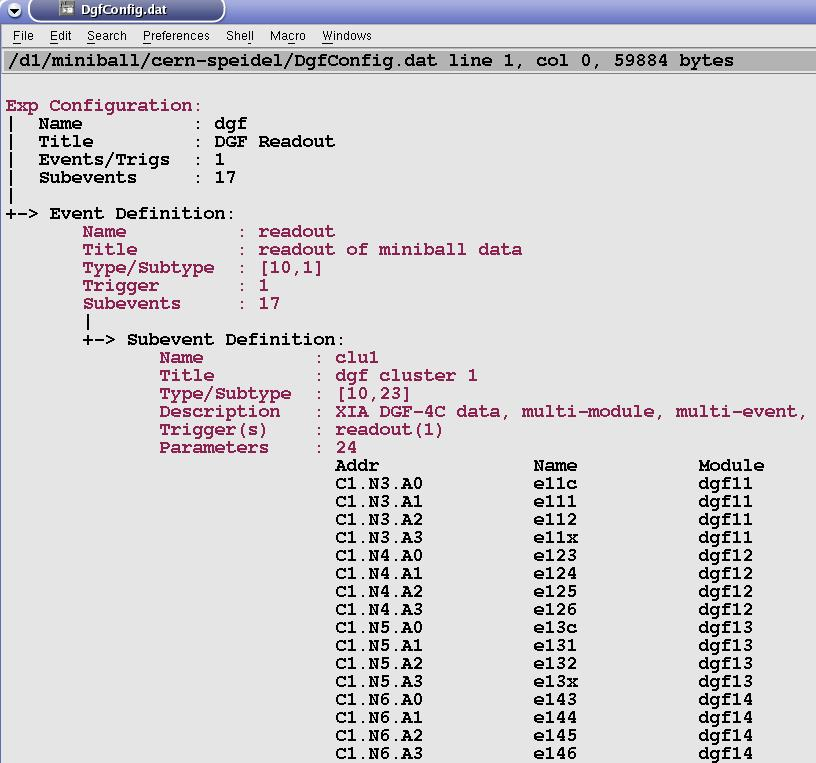
\includegraphics[width=\linewidth]{DgfConfig}}
\caption{\texttt{DgfConfig.dat}: printout of config data}
\label{DgfConfig}
\end{figure}
\newpage
\subsection{Various file formats}
\subsubsection{Cluster definition files}\label{ClusterDef}

The format of cluster definition files is adopted from Nigel Warr's Miniball Configuration sheet (fig.\ref{CluDef}).\\
\begin{figure}[H]
\centerline{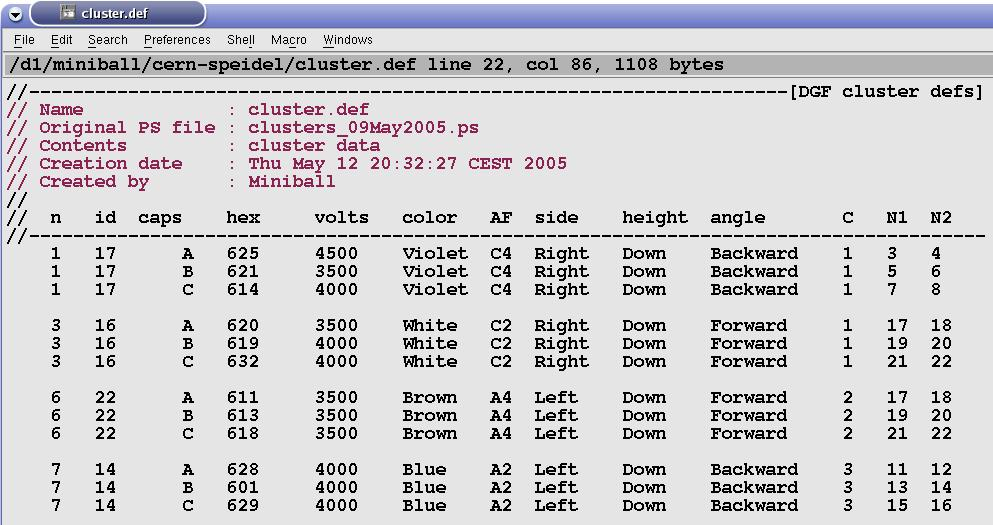
\includegraphics[width=\linewidth]{ClusterDef}}
\caption{\texttt{cluster.def}: define settings for DGF clusters}
\label{CluDef}
\end{figure}
\newpage
\subsubsection{Energy calibration file}\label{MBcalFileFormat}

An energy calibration file generated by \texttt{MBcal.C} is formatted usind the \texttt{ROOT} resource format.
It consists of a header followed by entries for each histogram.

\begin{center}
\begin{tabular}{|l|l|}
\hline
Header	&	\texttt{Calib.ROOTFile: <HistoFile>.root}		\\
	&	\texttt{Calib.Source: Co60 or Eu152 or TripleAlpha}		\\
	&	\texttt{Calib.NofHistograms: <N>}		\\
\hline
Entry	&	\texttt{Calib.<HistoName>.Xmin:	<Value>}	\\
(1 per histo) &	\texttt{Calib.<HistoName>.Xmax:	<Value>}	\\
	&	\texttt{Calib.<HistoName>.Gain: <Value>}	\\
	&	\texttt{Calib.<HistoName>.Offset: <Value>}	\\
\hline
\end{tabular}
\end{center}

\subsubsection{Doppler correction file}\label{DCorrFileFormat}

The dcorr file is formatted according to the \texttt{ROOT} resource format.
It consists of a header followed by entries for each histogram / each parameter.
\begin{itemize}
\setlength{\rightmargin}{1em}%
\setlength{\leftmargin}{2em}%
\setlength{\itemsep}{0pt}%
\setlength{\parskip}{1mm}%
\setlength{\partopsep}{0pt}%
\setlength{\parsep}{0pt}%
\setlength{\topsep}{0pt}%
\item	\yellow{Constant factor mode}\\
	\begin{center}
	\begin{tabular}{|l|l|}
	\hline
	Header	&	\texttt{DCorr.Type: ConstFactor}		\\
		&	\texttt{DCorr.NofHistograms: <N>}		\\
	\hline
	Entry	&	\texttt{DCorr.<HistoName>.Xmin:	<Value>}	\\
	(1 per histo) &	\texttt{DCorr.<HistoName>.Xmax:	<Value>}	\\
		&	\texttt{DCorr.<HistoName>.Factor: <Value>}	\\
	\hline
	\end{tabular}
	\end{center}
\item	\yellow{Fixed angle mode}\\
	\begin{center}
	\begin{tabular}{|l|l|}
	\hline
	Header	&	\texttt{DCorr.Type: FixedAngle}			\\
		&	\texttt{DCorr.NofHistograms: <N>}		\\
		&	\texttt{DCorr.AngleInDegrees: TRUE or FALSE}	\\
		&	\texttt{DCorr.Beta: <Value>}			\\
	\hline
	Entry	&	\texttt{DCorr.<HistoName>.Xmin:	<Value>}	\\
	(1 per histo) &	\texttt{DCorr.<HistoName>.Xmax:	<Value>}	\\
		&	\texttt{DCorr.<HistoName>.Angle: <Value>}	\\
	\hline
	\end{tabular}
	\end{center}
\item	\yellow{Particle-dependent angle mode}\\
	\begin{center}
	\begin{tabular}{|l|l|}
	\hline
	Header	&	\texttt{DCorr.Type: VariableAngle}		\\
		&	\texttt{DCorr.NofHistograms: <N>}		\\
		&	\texttt{DCorr.AngleInDegrees: TRUE or FALSE}	\\
	\hline
	Entry	&	\texttt{DCorr.<HistoName>.Xmin:	<Value>}	\\
	(1 per histo) &	\texttt{DCorr.<HistoName>.Xmax:	<Value>}	\\
		&	\texttt{DCorr.<HistoName>.Angle: <Value>}	\\
	\hline
	\end{tabular}
	\end{center}
\end{itemize}
\end{document}
